\documentclass[main.tex]{subfiles}
\newcommand\chapterlabel{kinetics}
\setcounter{figurenewcounter}{0}


\begin{document}
\linenumbers
%\setcounter{chapter}{5}
  
\chapter[Chemical kinetics]{Chemical kinetics}
%\label{ch:atoms}


      \begin{marginfigure}
      \begin{tikzpicture} \node (a) at (0,0) {\includegraphics[width=4cm]{chapter17/figure1}} node[rotate=90, font=\tiny] at ([yshift=.5cm,xshift=.1cm]a.south east) {\textsuperscript{\textcopyright} PxFuel} ;
\end{tikzpicture}
\end{marginfigure}


\lettrine[lines=4]{\color{black!45}T}{he} rate at which a chemical reaction occurs is a critical parameter at an industrial and laboratory-level as the faster the speed the sooner one can commercialize or sell a given chemical product. Slow chemical reactions are, in general, less desirable as it takes more time for the reagents to react. On the other hand, too fast chemical reactions can also be less desirable. Think, for example, in an explosion in which gas and a spark quickly generate carbon dioxide with water and a lot of heat in a way that is not easy to control. This chapter deals with the rate of reactions. You will learn how to calculate what we call a rate law which is a mathematical formula that gives the numerical rate value. You will also learn the collision theory that explains the factors that affect the speed of chemical reactions. 
\begin{marginfigure}%LEARNING GOALS BOX
\begin{mytcbox}{GOALS}
\begin{enumerate}[label=\protect\circled{\color{white}\arabic*}]
\item Analyze a rate law
\item Interconvert rates of reactants and products
\item Obtain rate laws
\item Compute activation energies
\item Analyze energy profiles
\end{enumerate}
\end{mytcbox}
\vspace{1cm}
\begin{tcolorbox}[enhanced,colback=red!5!white,colframe=black!50!red,boxrule=1pt,
  arc=0pt,outer arc=0pt,drop heavy lifted shadow]
\faGears\ 
\docenvdef{Discussion:} (a) \discussionKINETICSA (b) \discussionKINETICS \end{tcolorbox}
\end{marginfigure}%LEARNING GOALS BOX



\section{Rate of reaction}
Some chemical reactions are fast such as the explosive reaction between cooking gas and oxygen, happening almost instantaneously. Other reactions are slow such as the rusting of iron, taking months to occur. Chemical kinetics is a chemistry discipline that studies the speed of chemical reactions and the factors that affect this measure. The overall goal here is to understand the factors that control the rate of reactions with the ultimate goal of maximizing the generation of products. This section covers the principles of reaction rates, defining two different types of rates, and showing how to interconvert rates of reaction.
\sloppy 
\begin{description}
\item[\docfilehook{Two different ways of defining the reaction rate}{}] 
When a chemical reaction proceeds, reactants decompose into products. Therefore, the concentration of reactants decreases with time as reactant molecules become products, and the concentration of products increases with time as products are being formed. This change in concentration with time is what we call reaction rate. There are two different ways of defining the rate of a reaction. We can define the average reaction rate $\overline{r}$ as the change in concentration with time or as an instantaneous rate $r$ when the time interval is very small (we call this derivative):
\begin{equation}
\boxed{\overline{r}=\frac{\Delta c}{\Delta t} 
\quad  \text{or }\quad 
 r=\lim\limits_{\Delta t \to 0}     \frac{\Delta c}{\Delta t}=\frac{d c}{d t}}
\label{\chapterlabel:equation1}
\end{equation}
Both types of rates are not numerically the same. The average rate is an average change in concentration between two different times. At the same time, the time interval for the average can be large or small.
Differently, the instantaneous rate is calculated as the slope in the concentration vs. time plot at a given time--using mathematical terms we call this the derivative. Instantaneous rates represent more accurately the changes in concentration happening in a reaction. For this reason, from now on, whenever we describe a reaction rate we will refer to the instantaneous rate.
\item[\docfilehook{Rate of appearance and disappearance}{}] 
At the beginning of a reaction, the molecules of reactants will be consumed while the molecules of products will form. There are three different ways to measure the reaction rate. We can measure the amount of reactants that disappear per unit of time and this would give you the rate of disappearance of a reactant. We can also measure the amount of products formed per unit of time and that would give you the rate of appearance of a  product. As a note, rates of disappearance are negative (as the molarity of reactants decreases with time) whereas rates of appearance are positive. Finally, we can measure the amount of reactants the interconvert into products and that would give you the overall rate of reaction, which is always a positive number. Overall, by measuring concentration changes of reactants and products we can compute three types of rates: rates of disappearance, rates of appearance, and rates of reaction.

    \stepcounter{figurenewcounter}   \refstepcounter{figure}  \label{Fig:{\chapterlabel}\thefigurenewcounter}
     \begin{center}
    \pgfkeys{tikz/.cd,
tangent length/.store in=\TangentLength,
tangent length=7mm,
normal length/.store in=\NormalLength,
normal length=7mm}
\tikzset{tangent/.style={red,thin},normal/.style={red,thin},
tangent at/.style={postaction={decorate,decoration={markings,
mark=at position #1 with {\draw[tangent,shift={(0,1.60em-1.6em)}, rotate=-0] (-2*\TangentLength,0) -- (0.4*\TangentLength,0)   -- ++ (-4.7em,-0.6em) -- cycle; \node[shift={(-2em,1em)}, red] (-\TangentLength,0) {$r$} node[shift={(-4.4em,.3em)}, red] (-\TangentLength,0) {\tiny $d$c} node[shift={(-2em,-.2em)}, red] (-\TangentLength,0) {\tiny $d$t};
\fill[tangent,shift={(0,1.60em-1.6em)}]  (-\TangentLength,0) circle (1pt);}}}},
%normal at/.style={postaction={decorate,decoration={markings,
%mark=at position #1 with {\draw[normal] (0,-\NormalLength) -- (0,\NormalLength);
%\fill[normal] (0,0) circle (2pt);}}}},
}
\begin{tikzpicture}
  \begin{axis}[
            axis lines=middle,
             enlargelimits=0.1,
            xmin=0,
            xmax=1.0,
            ymin=0.01,
            ymax=0.1,
            xtick=\empty,
            ytick=\empty,xtick distance=0.05,
            xlabel=$\text{time}$,
            ylabel=$c\text{, M}$,
            x label style={at={(axis description cs:0.5,-0.0)},anchor=north},
    y label style={at={(axis description cs:0.07,.4)},rotate=90,anchor=south},
             domain=\pgfkeysvalueof{/pgfplots/xmin}:(\pgfkeysvalueof{/pgfplots/xmax},
            tangent/.style={add node at x={#1}{},},
        ]
     	              
            \addplot [thick,draw=blue!75!black, tangent at/.list={ 0.8 }]{0.1*exp(-2.9*x)};
                         \addplot [blue!75!black, mark=*,  draw=none , samples=5 ]{0.1*exp(-2.9*x)};
	 \draw[red] (6.4em,6em+0.8em) --++(0em,-3.5em+0.1em)--++(6.1em,0em ) -- cycle ;
	 \node[shift={(8.5em,5.5em+0.7em)}] (0,0) {$\overline{r}$} node[shift={(5.5em,5em+0.7em)}] (0,0) {\tiny $\Delta c$} node[shift={(8.5em,2.0em+0.9em)}] (0,0) {\tiny $\Delta t$} node[green!75!black, shift={(23em,12em)}] (0,0) {\small Product} node[blue!75!black, shift={(23em,2em)}] (0,0) {\small Reactants} ; 
                \addplot  [thick,draw=green!75!black]{0.1*(1-exp(-2.9*x))};
	             \addplot  [green!75!black, mark=*,  draw=none , samples=5]{0.1*(1-exp(-2.9*x))}; 


        \end{axis}
     \begin{scope}[xshift =0em, yshift =0em]
\node[text width=12cm, fontscale=0.1, shift={(15em,-4em)}] at (-0em,-0em) { \begin{bf}\color{black}\bfseries\large Figure \ref{Fig:{\chapterlabel}\thefigurenewcounter} \end{bf} Change of the concentration of reactants and products with time showing the average and instantaneous velocity.  };
   \end{scope} 
\end{tikzpicture}\end{center}

Let us work on a sample reaction:
\begin{center}\ce{I^-_{(aq)} + OCl^-_{(aq)} -> Cl^-_{(aq)} + OI^-_{(aq)}}\end{center}
We can think of the rate of disappearance of \ce{I^-_{(aq)}} that should be written as:
\[r_{\ce{I^-}} =  \frac{d\ce{\text{[\ce{I^-}]}}}{d t}\]
Similarly, we have that the rate of appearance of \ce{Cl^-} is:
\[r_{\ce{Cl^-}} =  \frac{d\ce{\text{[\ce{Cl^-}]}}}{d t}\]
As chemical rates represent the change of concentration of a given reactant with time, the units for a chemical rate are M/s.
\item[\docfilehook{Relating rates of appearance and disappearance}{}] 
We can relate the rates of any two reactants or products in a chemical reaction and, at the same time, we can relate the rate of reaction with the rate of any product or reactant--remember there is a single rate of reaction and multiple rates of appearance and disappearance of products and reactants. For example, for the following reaction:
\begin{center}\ce{4NH3_{(g)} + 5O2_{(g)} -> 4NO_{(g)} + 6H2O_{(g)}}\end{center}
We can relate $r_{\ce{NH3}}$ and $r_{\ce{H2O}}$:
\[-\frac{1}{4}r_{\ce{NH3}}=+\frac{1}{6}r_{\ce{H2O}}\]
Overall, a negative sign should be included before the rate of any reactant and a positive sign before the rate of any product. You also need to divide by the stoichiometric coefficients of each reactant and product. Similarly, we can relate $r_{\ce{O2}}$ with the rate of reaction $r$:
\[-\frac{1}{5}r_{\ce{O2}}= r \]
For a general equation such as:
\begin{center}\ce{aA + bB -> cC + dD}\end{center}
we have that the general relationship between any rate and the overall reaction rate is:
\begin{equation}
\boxed{r=-\frac{1}{a}r_A=-\frac{1}{b}r_B=+\frac{1}{c}r_C=+\frac{1}{d}r_D  }
\label{\chapterlabel:equation2}
\end{equation}
\begin{example} %%%%%%%%%%%%%%%%%%%%%%%% EXAMPLE BOX
For the reaction below, the rate of disappearance of A is -0.1M/s. Calculate:
\begin{inparaenum}[(a)]	
\item The rate of disappearance of B.
\item	 The rate of appearance of C.
\item  The rate of appearance of D.
\item  The rate of reaction.
\end{inparaenum} 
\begin{center}\ce{2A + 3B -> 4C + 5D}\end{center}
\textlcsc{ \textcolor{dgreen}{\Large \textbf{Solution}} }\\
In order to calculate the rate of disappearance of B, we will use the following relationship, in which the rate of disappearance of A and B have a negative sign and carries the respective stoichiometric coefficient
\[-\frac{1}{2}r_A=-\frac{1}{3}r_B\]
We know $r_A$ and hence we can solve for $r_B$:
\[-\frac{1}{2}(-0.1)=-\frac{1}{3}r_B\]
We have that $r_B$ is -0.15M/s. We will now use a similar relationship to calculate $r_C$:
\[-\frac{1}{2}(-0.1)=+\frac{1}{4}r_C\]
We have that $r_C$ is +0.2M/s. Finally, we will calculate $r_D$ and $r$:
\[-\frac{1}{2}(-0.1)=+\frac{1}{5}r_D \text{ and } -\frac{1}{2}(-0.1)=r\]
We have that $r_D$ is +0.25M/s and $r$ is 0.05M/s. Mind the rate of disappearance of reactants are negative, whereas the rate of appearance of products and the overall rate of reaction are positive numbers.
\\\faDiamond\ \textlcsc{ \textcolor{dgreen}{\Large \textbf{Study Check}} }\\
For the reaction below, the rate of appearance of C is 0.3M/s. Calculate:
\begin{inparaenum}[(a)]	
\item The rate of disappearance of A and B.
\item  The rate of appearance of D.
\item  The rate of reaction.
\end{inparaenum} 
\begin{center}\ce{5A + 2B -> C + 2D         }\end{center}
\flushright Answer:  $r_A$=-1.5M/s, $r_B$=-0.6M/s, $r_D$=0.6M/s, and $r$=0.3M/s
\end{example}%%%%%%%%%%%%%%%%%%%%%%%% EXAMPLE BOX
\end{description}

\section{Rate law}
Some chemical reactions double their rate by increasing the concentration of reactants, whereas, for the same change of concentration, others quadruple their rate. The rate law of a reaction is an experimental formula that explicitly includes the power dependence of the rate of reaction on the concentration of reactants and products. You can find rate laws in a differential form and in an integrated form. 
 On one hand, the differential rate law, or simply the rate law, is convenient when we want to assess the impact of concentration on the rate of reaction. On the other hand, integral rate laws give the time dependency of the concentration, being convenient to track how the reactants disappear with time. This section will cover how to interpret rate laws and how to differentiate rate laws from integral rate laws. It will also introduce the concept of the partial and the total order of reaction, as well as the idea of reaction rate constant.\sloppy 
\begin{description}
\item[\docfilehook{The rate law}{}] 
The rate law is an experimental expression, a formula that comes from an experiment, relating the rate of reaction with the concentration of the chemicals that impact the rate. An example of a rate law would be:
\[r=k[\ce{NO}]^2[\ce{O2}]\]
where:
\begin{where}
 \item $r$   is the overall rate of reaction
  \item $k$ is the rate constant 
 \item $[\ce{NO}]$  is the molarity of \ce{NO}
  \item $[\ce{O2}]$  is the molarity of \ce{O2}
\end{where}
So, what is the purpose of a rate law? Let us use the following rate law as an example:
\[r=0.002[\ce{NO}]^2[\ce{O2}]\]
By means of the rate law above, we can compute the numerical value of the rate of reaction for different concentrations. As such, rate laws help predict the value of the reaction rate. 



\item[\docfilehook{Partial and overall reaction orders}{}] 
The powers in the rate law are called reaction order. For example, in the rate law below
\[r=k[\ce{NO}]^2[\ce{O2}]\]
the order of \ce{NO} is $2$ as the power of \ce{NO} in the rate law is 2. Similarly, the partial order of \ce{O2} is $1$ as the power of \ce{O2} in the rate law is 1. The overall reaction order it 3, and this number results in adding all partial orders. Regarding the way we describe the reaction order, if the reaction order is one, we would say that the reaction is first order. Similarly, if the reaction order is two, we would say the reaction is second order, and so on. The reaction order can also be zero when the power in the rate law is zero. Reaction orders tend to be integer numbers such as 0, 1, or 2, mostly in educational problems. However, using realistic kinetic data, the partial and total orders can be any number and even have a negative sign. The reaction orders are very important as they indicate how the reaction rate responds to changes in concentration. For example, using the rate law above, if we double the concentration of \ce{O2} the rate law will double, but if we double the concentration of \ce{NO}, the reaction rate would quadruple, that is, it would be four times larger.
\item[\docfilehook{The rate constant, k}{}] 
The rate constant is a critical parameter of a rate law as it tells how the reaction responds to changes on molarity. For example, look this two different rate laws:
\[r_A=0.01[\ce{N2O5}]\quad\quad \text{ and } \quad\quad r_B=0.001[\ce{N2O5 }]\]
We have that as the rate constant in $r_A$ is larger the changes in the concentration of \ce{N2O5} will have a stronger impact on the rate than in  $r_B$. 

\begin{example} %%%%%%%%%%%%%%%%%%%%%%%% EXAMPLE BOX
Given the following rate law. Indicate:
\begin{inparaenum}[(a)]	
\item The rate constant giving the correct units.
\item	 The partial order of all species.
\item  The total order of the reaction.
\item  If $[\ce{F2}]$ is doubled how would the reaction rate be affected?
\end{inparaenum} 
\begin{center}\[r=0.002[\ce{Cl2}][\ce{F2}]^3\]\end{center}
\textlcsc{ \textcolor{dgreen}{\Large \textbf{Solution}} }\\
Given the information provided in the rate law, we have that the reaction is first order with respect to \ce{Cl2} and third order with respect to \ce{F2}. The overall reaction order is four. The rate constant is 0.002 1/$\text{M}^2$s.
\\\faDiamond\ \textlcsc{ \textcolor{dgreen}{\Large \textbf{Study Check}} }\\
Given the following rate law. Calculate:
\begin{inparaenum}[(a)]	
\item The rate constant giving the correct units.
\item	 The partial order of all species.
\item  The total order of the reaction.
\item  If $[\ce{F2}]$ is doubled how would the reaction rate be affected?
\end{inparaenum} 
\begin{center}\[r=0.056[A]^4[B]^2[C]^2\]\end{center}
\flushright Answer:   Orders: A(4), B(2), C(2), overall(8); k=0.056 1/$\text{M}^7$s
\end{example}%%%%%%%%%%%%%%%%%%%%%%%% EXAMPLE BOX

The units of a rate constant are determined by the reaction order. In other words, given a reaction order, we will have a given unit for the rate constant. At the same time, given the units of a rate constant, we can also determine the order of the reaction. The following formula gives the constant units for a given reaction order $n$:
\begin{equation}
\boxed{\frac{M^{1-n}}{s} }
\label{\chapterlabel:equation3}
\end{equation}
where:
\begin{where}
 \item $n$   is the reaction order
\end{where}
For example, for first-order reaction ($n$=1) the units of the reaction constant are 1/s and for a second-order reaction, the units are 1/Ms. For a reaction of zero-order, the units of the constant are M/s. This formula results from a dimensional analysis given that the units of reaction rate $r$ are M/s and the units of concentration is molarity, M. As a side note, here we will use second as a unit of time, however, one can envision a similar formula for different time units.
\begin{example} %%%%%%%%%%%%%%%%%%%%%%%% EXAMPLE BOX
Given the following rate constants indicate the reaction order:
\begin{inparaenum}[(a)]	
\item  $k$=0.04 M/s
\item	 $k$=0.09 1/Ms 
\item  $k$=0.03 /M$^4$s
\end{inparaenum} \\
\textlcsc{ \textcolor{dgreen}{\Large \textbf{Solution}} }\\
We will use Formula \ref{\chapterlabel:equation3} to calculate the reaction order. We have that 0.04 M/s is order zero, 0.09 1/Ms is first order and 0.03 /M$^4$s is fifth order.
\\\faDiamond\ \textlcsc{ \textcolor{dgreen}{\Large \textbf{Study Check}} }\\
Given the following rate constants indicate the reaction order:
\begin{inparaenum}[(a)]	
\item $k$=0.03 1/s
\item	 $k$=$3\times 10^{-4}$ L/smol
\item  $k$=$3\times 10^{-5}$ 1/sM$^2$
\end{inparaenum} 
\flushright Answer:   
\begin{inparaenum}[(a)]	
\item Order 1
\item	 Order 2
\item  Order 3
\end{inparaenum}
\end{example}%%%%%%%%%%%%%%%%%%%%%%%% EXAMPLE BOX

\item[\docfilehook{Integral reaction law}{}] 
The reaction law is more specifically called a differential reaction law as it represents a differential equation--this is a mathematical term to describe equations in terms of derivatives. For a differential rate law, there is an integral rate law. The integral rate law is obtained using a mathematical technique called integration--this technique is out of the scope of this class. For example, below we have an example of a differential and integral rate law for a first-order reaction.
\begin{center}$r =0.01[\ce{N2O5}]$ \hspace{1cm}and\hspace{1cm} $\text{Ln}[\ce{N2O5}]=-0.01\cdot t+\text{Ln}(0.1)$\end{center}
In the differential rate law, we have the explicit reaction rate $r$ accompanied by molarities ([\ce{N2O5}]), whereas in the corresponding integral rate law we have molarities ([\ce{N2O5}]) accompanied of time. The integral rate law gives the change of the concentration with time, whereas the differential rate law gives the change of the reaction rate with concentration. Each type of law has its purpose and differential rate laws are more common and used when we have experimental data in terms of reaction rates and molarities. The integrated rate law is used when we have data in terms of molarity and time. Overall, differential rate laws and integral rate laws are exchangeable. To convert a differential rate law into its corresponding integral rate law we just need the initial concentration of the species involved in the law, $[\ce{A}]_0$. For example, the corresponding differential and integral rate law for a zeroth-order reaction are:
 \begin{center}
\refstepcounter{table}  \label{tab:{\chapterlabel}1}
\fontfamily{ppl}\selectfont
\begin{tabular}{llll}
\rowcolor{black!45}
\toprule
\multicolumn{4}{l}{\hypersetup{colorlinks,linkcolor={white}} \cellcolor{black}\color{white}\bfseries\small Table \ref{tab:{\chapterlabel}1} Corresponding differential, integral rate laws and half-life formulas } \\
\midrule
 \rowcolor{gray!10} Order & Differential rate law & Integral rate law & Hal-life ($t_{\nicefrac{1}{2}}$) formula\\
\midrule
 0	& \multicolumn{1}{c}{	$r=k$	}&\multicolumn{1}{c}{$	[\ce{A}] =-k\cdot t + [\ce{A}]_0$	} &\multicolumn{1}{c}{$\frac{[\ce{A}]_0}{2k}$	} \\ [5mm]
 1	& \multicolumn{1}{c}{	$r=k[A]$	}&\multicolumn{1}{c}{$	\text{Ln}[\ce{A}]=-k\cdot t+\text{Ln}[\ce{A}]_0	$	} &\multicolumn{1}{c}{$\frac{0.693}{k}$	} \\ [5mm]
  2	& \multicolumn{1}{c}{	$r=k[A]^2$	}&\multicolumn{1}{c}{$	\frac{1}{[\ce{A}]}=k\cdot t +\frac{1}{[\ce{A}]_0}$	} &\multicolumn{1}{c}{$\frac{1}{k[\ce{A}]_0}$	} \\ [5mm]
 \bottomrule
\end{tabular}\end{center} 
Table \ref{tab:{\chapterlabel}1} reports the corresponding differential and integral rate laws for different orders.
\begin{example} %%%%%%%%%%%%%%%%%%%%%%%% EXAMPLE BOX
Identify the following rate law as differential or integral and switch into the other form.
\begin{center}\[\frac{1}{[\ce{C2H6}]}=4\times 10^{-4}\cdot t +\frac{1}{0.03}\]\end{center}
\textlcsc{ \textcolor{dgreen}{\Large \textbf{Solution}} }\\
As the equation contains time this would be a integrated rate law. We can use Table \ref{tab:{\chapterlabel}1} to identify the order and compute the differential law. This is a first order reaction with rate constant $4\times 10^{-4}$ 1/s, therefore:
\[r=  4\times 10^{-4} [\ce{C2H6}] \]
\\\faDiamond\ \textlcsc{ \textcolor{dgreen}{\Large \textbf{Study Check}} }\\
Identify the following rate law as differential or integral and switch into the other form for an initial concentration of 0.3M.
\begin{center}\[r=5\times 10^{-2}\]\end{center}
\flushright Answer:   $[\ce{A}] =-5\times 10^{-2}\cdot t + 0.3$
\end{example}%%%%%%%%%%%%%%%%%%%%%%%% EXAMPLE BOX

\item[\docfilehook{Half-life, $t_{\nicefrac{1}{2}}$}{}] 
When a reaction starts to happen, the concentration of reactants decreases with time. Half-life is the time at which the initial concentration of reactants is half its initial value. Reactions with small half-life are fast, as they take a short time to reduce the concentration of reactants to half. Differently, reactions with large half-life are slow as they need longer times to proceed. This way, the numerical value of half-life helps you compare the speed of reactions. At the same time, the half-life is a transformation of the rate constant into a time value. That is, by rate constants can be converted into half-lives.
There is a single half-life formula for each reaction order and Table \ref{tab:{\chapterlabel}1} reports some half-life formulas. 
If you wonder, where these formulas come from, one can obtain all these formulas by using $[A]=[A]_0/2$ in any integral rate law. For example, for a first order reaction we have that:
\[\text{Ln}[\ce{A}]=-k\cdot t+\text{Ln}[\ce{A}]_0 \]
When $[A]=[A]_0/2$ we have that $t=t_{\nicefrac{1}{2}}$ and therefore:
\[\text{Ln}\Bigg(\frac{[A]_0/2}{[\ce{A}]_0}\Bigg)=-k\cdot t_{\nicefrac{1}{2}}\] that leads to
\[t_{\nicefrac{1}{2}}=-\frac{\text{Ln}(0.5)}{k} \]\begin{example} %%%%%%%%%%%%%%%%%%%%%%%% EXAMPLE BOX
Calculate the half-life for a second order reaction with initial concentration of $5.99\times 10^3$ M if the rate constant is 0.005 1/Ms? 
\\
\textlcsc{ \textcolor{dgreen}{\Large \textbf{Solution}} }\\
As we deal with a second order reaction, we will use $\frac{1}{k[\ce{A}]_0}$ given that $[\ce{A}]_0=5.99\times 10^3$M and $k$=0.005 1/Ms. We have that
\[t_{\nicefrac{1}{2}}=\frac{1}{0.005\cdot 5.99\times 10^3}=0.03s\]
\faDiamond\ \textlcsc{ \textcolor{dgreen}{\Large \textbf{Study Check}} }\\
Calculate the half-life for a first order reaction with initial concentration of $5.99\times 10^3$ mol/L if the rate constant is 0.02 1/s? \\
\flushright Answer:   3.465s
\end{example}%%%%%%%%%%%%%%%%%%%%%%%% EXAMPLE BOX
\end{description}
\section{The differential and integral methods for obtaining rate laws}
Up to now, we analyzed the importance of using rate laws. However, before this point, all rate laws were given. This section will cover how to experimentally obtain rate laws by analyzing experimental data. There are two main methods for obtaining rate laws: the differential method and the integral method and each method differs not only on the nature of the experimental data gathered but also on how this data is processed. 
\sloppy 
\begin{description}
\item[\docfilehook{The differential method}{}] 
The differential method also called the method of the initial rates measures velocities for different concentrations, and in particular, measures initial velocities. These are velocities at very short times after the reaction starts. This method is convenient when there are parasite reactions that compete with the reaction one wants to study. By using initial rates, we can minimize the impact of competing reactions on the kinetic data.
In this method, by comparing different velocities for different concentrations one can calculate the reaction order and the rate constant, that is, one can construct the rate law. The next example will show you how to use this method. As a note, one can only use the differential method when reaction rates data is supplied.
\begin{example} %%%%%%%%%%%%%%%%%%%%%%%% EXAMPLE BOX
Use the data below to calculate the rate law of the following reaction: \begin{center}\ce{A -> B}\end{center}
\begin{center}\begin{tabular}[t]{  c c  c   }
\toprule
 Experiment &$r$ (M/s)	&$[A]$, (M) \\
\midrule
1&	0.5&	0.5\\
2&	0.72 &0.6	\\
\bottomrule
\end{tabular}\end{center}
\textlcsc{ \textcolor{dgreen}{\Large \textbf{Solution}} }\\
As they provide values of $[A]$ the rate law should be $r=k[A]^n$. In order to calculate the rate law we need the values of $k$ and $n$.
We will apply the rate law two the two different experiments and divide:
\begin{align*}
&\
   \left.\begin{aligned}
    0.5=k0.5^n\quad (\text{Experiment 1}) \\
    0.72=k0.6^n\quad (\text{Experiment 2}) 
\end{aligned}
\right\}         \frac{0.5}{0.72}=\frac{\cancel{k}}{\cancel{k}}\cdot \Bigg(\frac{0.5}{0.6}\Bigg)^n 
\end{align*}
This approach will cancel $k$ leaving only $n$. 
\[ 0.694=(0.833)^n\]
Remember that if we divide two numbers with the same exponent we can combine the numbers and share the exponents. In order to solve for $n$ we need to apply 	natural logarithms (or simply log) to both sides of the equation in order to move the exponent down:
\[Ln(0.694)=n\cdot Ln(0.833) \text{that gives }n=\frac{Ln(0.694)}{Ln(0.833)}=1.99=2\]
Remember the orders are normally integer numbers so you can round to the closes integer. Now that we have the order, we can use the rate law again to obtain the rate constant using for example: $r$=0.5M/s and $[A]=$0.5M, and given that now we know $n$=2
\[ 0.5=k0.5^2\]
Solving for $k$ we have $k$=2 1/Ms. We have that the reaction law is: $r=2[A]^2$
\\
\faDiamond\ \textlcsc{ \textcolor{dgreen}{\Large \textbf{Study Check}} }\\
Use the data below to calculate the rate law of the following reaction: \ce{A -> B}
\begin{center}\begin{tabular}[t]{  c c  c   }
\toprule
 Experiment &$r$ (M/s)	&$[A]$, (M) \\
\midrule
1&	0.5&	2.5\\
2&	0.6 &3.0	\\
\bottomrule
\end{tabular}\end{center}
\flushright Answer:   $r=0.2[A]^1$
\end{example}%%%%%%%%%%%%%%%%%%%%%%%% EXAMPLE BOX
This previous example was useful to obtain the rate law using data involving only the concentration of one reactant. In other words, the previous example was useful to obtain simple rate law such as:
\[r=k[A]^x\]
The next example will cover how to calculate the rate law when the data provided involved the concentration of two reactants and therefore the rate law contains the orders of two species. In other words, the next example will show how to obtain more complex rate laws such as:
\[r=k[A]^x[B]^y\]
in which we do not know the reaction constant and two of the order.
\begin{example} %%%%%%%%%%%%%%%%%%%%%%%% EXAMPLE BOX
Use the data below to calculate the rate law of the following reaction: \ce{A + B -> C}
\begin{center}\begin{tabular}[t]{  c c  c c  c  }
\toprule
Experiment	&$[A]$ (M)&		$[B]$ (M)	&	$r$ (M/s)\\
\midrule
1&	0.5&	0.2&	0.25\\
2&	0.6&	0.2&	0.36\\
3&	0.5&	0.3&	0.375\\
4&	0.6	&0.3	&0.54\\
\bottomrule
\end{tabular}\end{center}
\textlcsc{ \textcolor{dgreen}{\Large \textbf{Solution}} }\\
As they provide values of $[A]$ and  $[B]$ the rate law should be $r=k[A]^n[A]^m$. In order to calculate the rate law we need the values of $k$, $n$ and $m$.
We will apply the rate law two the two different experiments and divide. But this time we will sort the data appropriately. In order to calculate the order or A we will select the data with different values of $[A]$ and the same value of $[B]$:
\begin{center}\begin{tabular}[t]{  c c  c c  c  }
\toprule
Experiment	&$[A]$ (M)&		$[B]$ (M)	&	$r$ (M/s)\\
\midrule
1&	0.5&	0.2&	0.25\\
2&	0.6&	0.2&	0.36\\
\bottomrule
\end{tabular}\end{center}
Again, we will apply the rate law to each Experiment:
\begin{align*}
&\
   \left.\begin{aligned}
    0.25=k0.5^n0.2^m\quad (\text{Experiment 1}) \\
     0.36=k0.6^n0.2^m\quad (\text{Experiment 2}) 
\end{aligned}
\right\}         \frac{0.25}{0.36}=\frac{\cancel{k}}{\cancel{k}}\cdot \Bigg(\frac{0.5}{0.6}\Bigg)^n \cdot \Bigg(\frac{\cancel{0.2}}{\cancel{0.2}}\Bigg)^m   
\end{align*}
This approach will cancel $k$ and $[B]$ leaving only $n$ giving
\[0.694=(0.833)^n\]
In order to solve for $n$ we need to apply 	natural logarithms (or simply log) to both sides of the equation in order to move the exponent down:
\[Ln(0.694)=n\cdot Ln(0.833) \text{that gives }n=\frac{Ln(0.694)}{Ln(0.833)}=1.99=2\]
Again, remember the orders are normally integer numbers so you can round to the closes integer. 
In order to calculate the order or B we will select the data with different values of $[B]$ and the same value of $[A]$:
\begin{center}\begin{tabular}[t]{  c c  c c  c  }
\toprule
Experiment	&$[A]$ (M)&		$[B]$ (M)	&	$r$ (M/s)\\
\midrule
1&	0.5&	0.2&	0.25\\
3&	0.5&	0.3&	0.375\\
\bottomrule
\end{tabular}\end{center}
Again, we will apply the rate law to each Experiment:
\begin{align*}
&\
   \left.\begin{aligned}
   0.25=k0.5^n0.2^m\quad (\text{Experiment 1}) \\
     0.375=k0.5^n0.3^m\quad (\text{Experiment 3}) 
\end{aligned}
\right\}         \frac{0.25}{0.375}=\frac{\cancel{k}}{\cancel{k}}\cdot \Bigg(\frac{\cancel{0.5}}{\cancel{0.5}}\Bigg)^n \cdot \Bigg(\frac{ 0.2}{ 0.3}\Bigg)^m  
\end{align*}
We have that $0.666=(0.66)^m$.
The order of B is $m$=1. 
Now that we have the order, we can use the rate law again to obtain the rate constant using any of the experiments: 
\[0.25=k0.5^2 0.2^1\quad (\text{Experiment 1})\]
$r$=0.5M/s and $[A]=$0.5M, and given that now we know $n$=2
\[ 0.5=k0.5^2\]
Solving for $k$ we have $k$=5 1/M$^2$s. We have that the reaction law is: $r=5[A]^2[B]^1$
\\
\faDiamond\ \textlcsc{ \textcolor{dgreen}{\Large \textbf{Study Check}} }\\
Use the data below to calculate the rate law of the following reaction: \ce{A + B -> C}
\begin{center}\begin{tabular}[t]{  c c  c c  c  }
\toprule
Experiment	&$[A]$ (M)&		$[B]$ (M)	&	$r$ (M/s)\\
\midrule
1&	0.5	&0.2	&$2\times 10^{-4}$\\
2&	0.6&	0.2&	2$\times 10^{-4}$\\
3&	0.5&	0.3&	$4.5\times 10^{-4}$\\
4&	0.6&	0.3&	$4.5\times 10^{-4}$\\
\bottomrule
\end{tabular}\end{center}
\flushright Answer:  $r=5[B]^2$
\end{example}%%%%%%%%%%%%%%%%%%%%%%%% EXAMPLE BOX
\vspace{3cm}
\item[\docfilehook{The integral method: an introduction}{}] 
The integral method is used to calculate the rate law if data reporting concentration and time are given. To understand the use of the integral method, it is convenient to learn more about integral rate laws. Let us analyze the integral rate law for a zeroth-order reaction:
\[[\ce{A}] =-k\cdot t + [\ce{A}]_0\]
If you look carefully you could notice that this integral rate law is indeed a linear relationship. The term $[\ce{A}]_0$  and $k$ are constants. Differently, the terms $\ce{A}]$ and $t$ are variables. Linear relationships are mathematical relationships with an independent variable represented in the horizontal axes and a dependent variable represented in the vertical axis. In the rate law above the independent variable is $t$ and the dependent variable is $[\ce{A}]$ and for every value of $t$ we would have a given value of $[\ce{A}]$. Moreover, $-k$ is the slope of the relationship, and $[\ce{A}]_0$ is the intersect. Let us analyze another integral rate law, this time for a first-order reaction:
\[\text{Ln}[\ce{A}]=-k\cdot t+\text{Ln}[\ce{A}]_0\]
we have that this law also represent a linear relationship as well, with $t$ as independent variable (the $x$) and $Ln([\ce{A}])$ as the dependent variable (the $y$). The slope is $-k$ and the intersect is $Ln([\ce{A}]_0)$. Overall, we have that all integral rate laws are linear relationship with $t$ as the $x$ and different properties as the $y$:  $[\ce{A}]$ for a zeroth-order, $Ln([\ce{A}])$ for a first-order reaction and $\frac{1}{[\ce{A}]}$ for a second-order reaction. We also have that the slope of the lines in absolute value always gives $k$. This information is summarized in the table below.
 \begin{center}
\refstepcounter{table}  \label{tab:{\chapterlabel}2}
\fontfamily{ppl}\selectfont
\begin{tabular}{llllll}
\rowcolor{black!45}
\toprule
\multicolumn{6}{l}{\hypersetup{colorlinks,linkcolor={white}} \cellcolor{black}\color{white}\bfseries\small Table \ref{tab:{\chapterlabel}2} The integral method } \\
\midrule
 \rowcolor{gray!10} Order & \multicolumn{1}{c}{$y$} & \multicolumn{1}{c}{$x$} & Slope& Slope Sign&Intersect\\
\midrule
 0	& \multicolumn{1}{c}{	$[\ce{A}]$	}&\multicolumn{1}{c}{$t$	} &\multicolumn{1}{c}{$-k$	}&\multicolumn{1}{c}{$-$	}& \multicolumn{1}{c}{$[\ce{A}]_0	$	}\\ 
  1	& \multicolumn{1}{c}{	$Ln([\ce{A}])$	}&\multicolumn{1}{c}{$t$	} &\multicolumn{1}{c}{$-k$	}&\multicolumn{1}{c}{$-$	}&\multicolumn{1}{c}{$Ln([\ce{A}]_0)	$	} \\ 
 2	& \multicolumn{1}{c}{	$\frac{1}{[\ce{A}]}$	}&\multicolumn{1}{c}{$t$	} &\multicolumn{1}{c}{$+k$}&\multicolumn{1}{c}{$+$	}&\multicolumn{1}{c}{$\frac{1}{[\ce{A}]_0}	$	}	 \\ 
 \bottomrule
\end{tabular}\end{center} 

The integral method is based on plotting some kinetic data, for example, concentration vs. time, and fitting the data into a linear relationship.
If the quality of the fit is good enough, by reading the slope of the line and the intersect one can compute the rate law that rules the reaction.
To associate the experimental data into a line we use linear regression, a statistical tool that gives the equation of the best line that fits the experimental data. At the same time, linear regression gives an estimate of the goodness of the fit through a regression parameter, $r$ or $r^2$, depending on the statistics software employed.
Overall, is good to keep in mind that every plot ($[A]$ vs. t, Ln$[A]$ vs. t or $1/[A]$ vs. t) is associated to a specific order.  
\item[\docfilehook{The integral method: associating a linear plot with an order}{}] 
The base of the integral method is to create three different plots: (a) $[\ce{A}]$ vs. $t$ (b) $\text{Ln}[\ce{A}]$ vs. $t$ and (c) $\frac{1}{[\ce{A}]}$ vs. $t$. In all plots, time is always indicated in the horizontal axis. Based on the data, only one of the plots will be the best linear plot with a  regression coefficient $r^2$ closer to one. The perfect linear plot will be associated with an order (here, either 0, 1, or 2). If the plot $[\ce{A}]$ vs. $t$ gives a perfect line the reaction will be zeroth-order. If the plot $Ln([\ce{A}])$ vs. $t$ gives a perfect line the reaction will be first order. If the plot $\frac{1}{[\ce{A}]}$ vs. $t$ gives a perfect line the reaction will be second-order. It is convenient to practice identifying the different plots and associating them with an order. The following example covers just that.
\begin{example} %%%%%%%%%%%%%%%%%%%%%%%% EXAMPLE BOX
The following plots results from processing kinetic data by means of the integral method. They are all perfect lines with $r^2$=0.99. Indicate the order of the reaction.
\begin{center}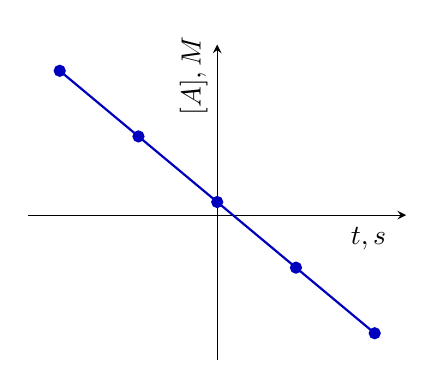
\begin{tikzpicture}
  \begin{axis}[
            axis lines=middle,
             enlargelimits=0.1,y=0.5cm/3,
    x=0.4cm,
%            xmin=0,
%            xmax=1.0,
%            ymin=0.01,
%            ymax=0.1,
            xtick=\empty,
            ytick=\empty,xtick distance=0.05,
            xlabel=$\text{t, s}$,
            ylabel=$\text{[A], M}$,
            x label style={at={(axis description cs:0.9,0.45)},anchor=north},
    y label style={at={(axis description cs:0.5,.9)},rotate=90,anchor=south},
%             domain=\pgfkeysvalueof{/pgfplots/xmin}:(\pgfkeysvalueof{/pgfplots/xmax},
        ]
            \addplot [thick,draw=blue!75!black]{-2*x+1};
                         \addplot [blue!75!black, mark=*,  draw=none , samples=5 ]{-2*x+1};
	        \end{axis}
	        
\end{tikzpicture}\hspace{0.5cm}\vspace{-0.6cm}
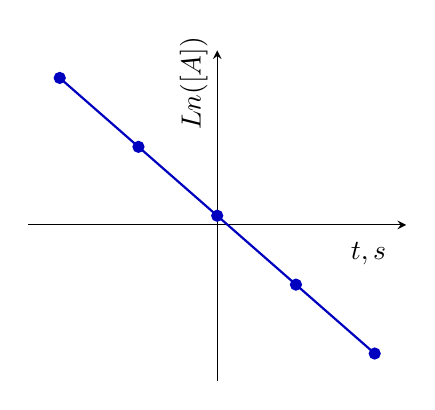
\begin{tikzpicture}
  \begin{axis}[
            axis lines=middle,
             enlargelimits=0.1,y=0.35cm/3,
    x=0.4cm,
%            xmin=0,
%            xmax=1.0,
%            ymin=0.01,
%            ymax=0.1,
            xtick=\empty,
            ytick=\empty,xtick distance=0.05,
            xlabel=$\text{t, s}$,
            ylabel=$\text{Ln([A])}$,
            x label style={at={(axis description cs:0.9,0.45)},anchor=north},
    y label style={at={(axis description cs:0.5,.9)},rotate=90,anchor=south},
%             domain=\pgfkeysvalueof{/pgfplots/xmin}:(\pgfkeysvalueof{/pgfplots/xmax},
        ]
            \addplot [thick,draw=blue!75!black]{-3*x+1};
                         \addplot [blue!75!black, mark=*,  draw=none , samples=5 ]{-3*x+1};
	        \end{axis}	        
\end{tikzpicture}
\end{center}
\textlcsc{ \textcolor{dgreen}{\Large \textbf{Solution}} }\\
We will inspect the linear plot and based on what is represented on the vertical and horizontal axis we will conclude the reaction order. The plot on the left represents molarity on the vertical axis and time on the horizontal. This is a zeroth-order reaction. On the other hand, the plot on the right represents the logarithm of molarity on the vertical axis and time on the horizontal axis. This is a first-order reaction.\\\faDiamond\ \textlcsc{ \textcolor{dgreen}{\Large \textbf{Study Check}} }\\
The following plots results from processing kinetic data by means of the integral method. They are all perfect lines with $r^2$=0.99. Indicate the order of the reaction.
\begin{center}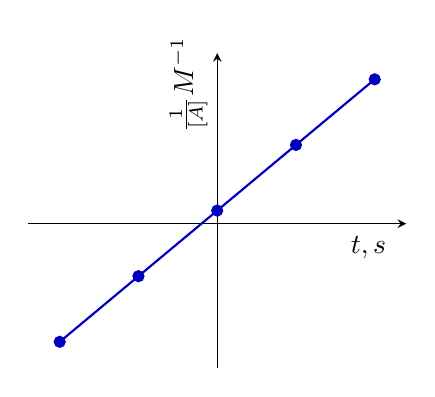
\begin{tikzpicture}
  \begin{axis}[
            axis lines=middle,
             enlargelimits=0.1,y=0.5cm/3,
    x=0.4cm,
%            xmin=0,
%            xmax=1.0,
%            ymin=0.01,
%            ymax=0.1,
            xtick=\empty,
            ytick=\empty,xtick distance=0.05,
            xlabel=$\text{t, s}$,
            ylabel=$\frac{1}{\text{[A]}}\text{M}^{-1}$,
            x label style={at={(axis description cs:0.9,0.45)},anchor=north},
    y label style={at={(axis description cs:0.5,.9)},rotate=90,anchor=south},
%             domain=\pgfkeysvalueof{/pgfplots/xmin}:(\pgfkeysvalueof{/pgfplots/xmax},
        ]
            \addplot [thick,draw=blue!75!black]{2*x+1)};
                         \addplot [blue!75!black, mark=*,  draw=none , samples=5 ]{2*x+1};
	        \end{axis}
	        
\end{tikzpicture}\hspace{0.5cm}\vspace{-0.6cm}
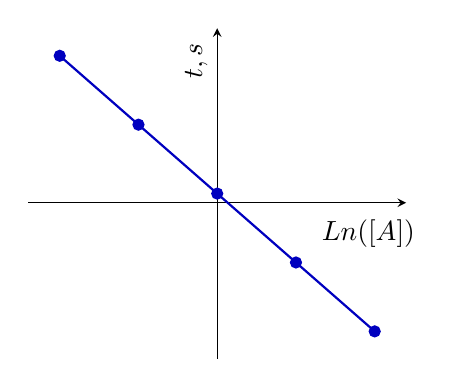
\begin{tikzpicture}
  \begin{axis}[
            axis lines=middle,
             enlargelimits=0.1,y=0.35cm/3,
    x=0.4cm,
%            xmin=0,
%            xmax=1.0,
%            ymin=0.01,
%            ymax=0.1,
            xtick=\empty,
            ytick=\empty,xtick distance=0.05,
            xlabel=$\text{Ln([A])}$ ,
            ylabel=$\text{t, s}$,
            x label style={at={(axis description cs:0.9,0.45)},anchor=north},
    y label style={at={(axis description cs:0.5,.9)},rotate=90,anchor=south},
%             domain=\pgfkeysvalueof{/pgfplots/xmin}:(\pgfkeysvalueof{/pgfplots/xmax},
        ]
            \addplot [thick,draw=blue!75!black]{-3*x+1)};
                         \addplot [blue!75!black, mark=*,  draw=none , samples=5 ]{-3*x+1};
	        \end{axis}
	        
\end{tikzpicture}
\end{center}\flushright Answer:   Left (order 2), right (order 1)
\end{example}%%%%%%%%%%%%%%%%%%%%%%%% EXAMPLE BOX

\item[\docfilehook{The integral method: extracting data from linear regressions}{}] 
We will practice the integral method by extracting the rate constant and the initial reactant concentration from the linear regression data. Linear regression software will give the equation of a line and the associated $r$ coefficient. We will have to read the slope and the intercept of the equation and infer the rate constant and the initial reactant concentration $[A]_0$.
The rate constant will be obtained from the slope of the line, whereas $[A]_0$ is related to the intercept.
For all cases, the absolute value of the slope of the line equation will correspond to the rate constant $k$. The relationship between $[A]_0$ and the intercept differs based on the order. For a zeroth-order plot, the intersect directly corresponds to the initial concentration. Differently, for a first-order reaction, the intercept corresponds to $Ln(\text{[A]}_0)$. Therefore, to obtain $[A]_0$ you will have to compute the exponential of the intersect: $[A]_0=\myexp{Intersect}$. Finally, for a second-order reaction, the slope will correspond to the inverse of the initial concentration, and hence, to obtain $[A]_0$ we will have to compute the inverse of the intersect: $[A]_0=\frac{1}{Intersect}$. The following example shows how to obtain the rate constant and $[A]_0$ using regression results.

\begin{example} %%%%%%%%%%%%%%%%%%%%%%%% EXAMPLE BOX
The following plots results from processing data by means of the integral method. Interpret the linear regressions and indicate the rate law.
\begin{center}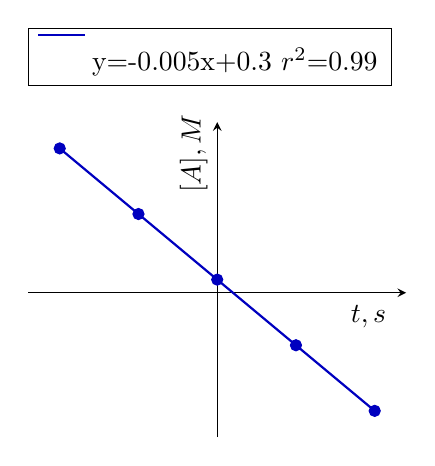
\begin{tikzpicture}
  \begin{axis}[
            axis lines=middle,legend style={at={(0.0,1.3)},anchor=north west} ,
             enlargelimits=0.1,y=0.5cm/3,
    x=0.4cm,
            xtick=\empty,
            ytick=\empty,xtick distance=0.05,
            xlabel=$\text{t, s}$,
            ylabel=$\text{[A], M}$,
            x label style={at={(axis description cs:0.9,0.45)},anchor=north},
    y label style={at={(axis description cs:0.5,.9)},rotate=90,anchor=south},
        ]
            \addplot [thick,draw=blue!75!black]{-2*x+1)};      
                                \addlegendentry[shift={(0,0em)}]{y=-0.005x+0.3 $r^2$=0.99  };
                         \addplot [blue!75!black, mark=*,  draw=none , samples=5 ]{-2*x+1};
	        \end{axis}
	        
\end{tikzpicture}\hspace{0.5cm}\vspace{-0.6cm}
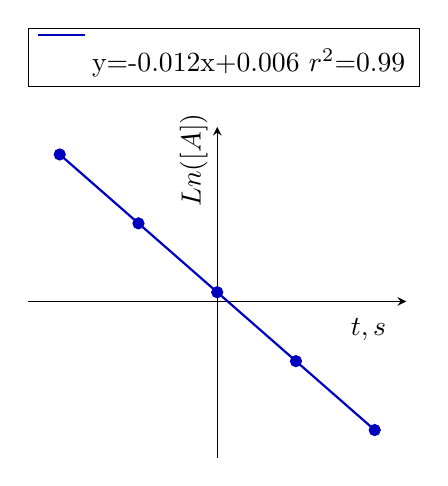
\begin{tikzpicture}
  \begin{axis}[
            axis lines=middle,legend style={at={(0.0,1.3)},anchor=north west} ,
             enlargelimits=0.1,y=0.35cm/3,
    x=0.4cm,
            xtick=\empty,
            ytick=\empty,xtick distance=0.05,
            xlabel=$\text{t, s}$,
            ylabel=$\text{Ln([A])}$,
            x label style={at={(axis description cs:0.9,0.45)},anchor=north},
    y label style={at={(axis description cs:0.5,.9)},rotate=90,anchor=south},
        ]
            \addplot [thick,draw=blue!75!black]{-3*x+1)};
                                            \addlegendentry[shift={(0,0em)}]{y=-0.012x+0.006 $r^2$=0.99  };

                         \addplot [blue!75!black, mark=*,  draw=none , samples=5 ]{-3*x+1};
	        \end{axis}
	        
\end{tikzpicture}
\end{center}
\textlcsc{ \textcolor{dgreen}{\Large \textbf{Solution}} }\\
We will inspect the linear regression to identify the reaction order. From the absolute value of the slope, we will obtain the rate constant. The plot from the left represents molarity and hence this is a zeroth-order reaction with a rate constant $k$=0.005M/s. The rate law would be: $r=0.005$. The plot from the right displays the logarithm of the concentration and hence this would be a first-order reaction, with a rate constant $k$=0.012 1/s. The rate law would be: $r=0.012\text{[A]}$. We can also calculate the initial concentration for each plot. On the left plot, we have that as this is a zeroth-order reaction the intercept directly gives you the initial concentration of reactants: $\text{[A]}_0$=0.3M. On the right plot, we have that as this is a first-order reaction the intercept gives you the logarithm of the initial concentration of reactants. We have that $Ln(\text{[A]}_0)$=0.006 and hence $\text{[A]}_0$=$e^{0.006}$=1.006M.\\\faDiamond\ \textlcsc{ \textcolor{dgreen}{\Large \textbf{Study Check}} }\\
The following plots results from processing data by means of the integral method. Interpret the linear regressions and indicate the rate law and the initial concentration of reactants.
\begin{center}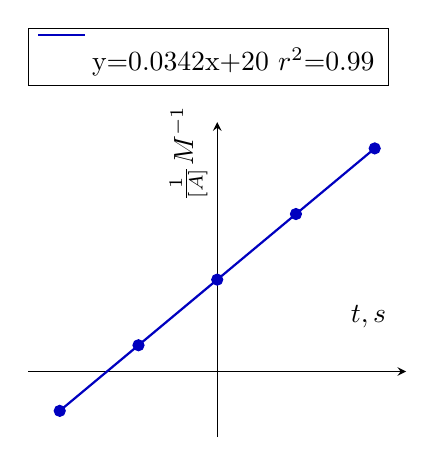
\begin{tikzpicture}
  \begin{axis}[
            axis lines=middle,legend style={at={(0.0,1.3)},anchor=north west} ,
             enlargelimits=0.1,y=0.5cm/3,
    x=0.4cm,
            xtick=\empty,
            ytick=\empty,xtick distance=0.05,
            xlabel=$\text{t, s}$,
            ylabel=$\frac{1}{\text{[A]}}\text{M}^{-1}$,
            x label style={at={(axis description cs:0.9,0.45)},anchor=north},
    y label style={at={(axis description cs:0.5,.9)},rotate=90,anchor=south},
        ]
            \addplot [thick,draw=blue!75!black]{2*x+7)};      
                                \addlegendentry[shift={(0,0em)}]{y=0.0342x+20 $r^2$=0.99  };
                         \addplot [blue!75!black, mark=*,  draw=none , samples=5 ]{2*x+7};
	        \end{axis}
	        
\end{tikzpicture}\hspace{0.5cm}\vspace{-0.6cm}
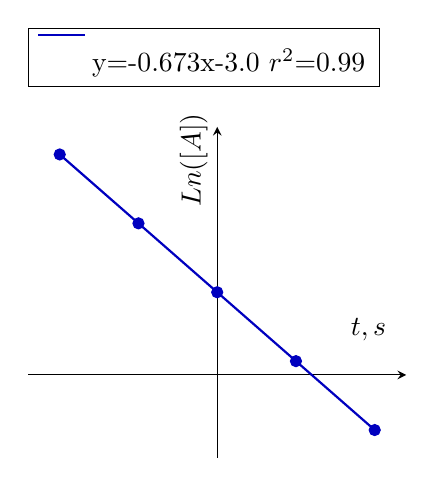
\begin{tikzpicture}
  \begin{axis}[
            axis lines=middle,legend style={at={(0.0,1.3)},anchor=north west} ,
             enlargelimits=0.1,y=0.35cm/3,
    x=0.4cm,
            xtick=\empty,
            ytick=\empty,xtick distance=0.05,
            xlabel=$\text{t, s}$,
            ylabel=$\text{Ln([A])}$,
            x label style={at={(axis description cs:0.9,0.45)},anchor=north},
    y label style={at={(axis description cs:0.5,.9)},rotate=90,anchor=south},
        ]
            \addplot [thick,draw=blue!75!black]{-3*x+9)};
                                            \addlegendentry[shift={(0,0em)}]{y=-0.673x-3.0 $r^2$=0.99  };

                         \addplot [blue!75!black, mark=*,  draw=none , samples=5 ]{-3*x+9};
	        \end{axis}
	        
\end{tikzpicture}
\end{center}\flushright Answer:   Left ($r=0.0342\text{[A]}^2$, $\text{[A]}_0$=0.05M), right ($r=0.673\text{[A]}$, $\text{[A]}_0$=0.05M)
\end{example}%%%%%%%%%%%%%%%%%%%%%%%% EXAMPLE BOX
\item[\docfilehook{The integral method in action}{}] 
Now we are ready to work from scratch on a set of data from the integral method. Normally, data involving concentration and time will be given. To apply the integral method, we need to process these data into three different columns, reporting the concentration, the logarithm of the concentration, and the inverse of the concentration. Next, we will do three plots and we will obtain the regression line for each plot. We will compare the goodness of the fit by assessing the value of $r^2$. The closer this value to one the better the fit. This analysis will lead to the reaction order. Finally, after we have selected the plot that corresponds to the best fit, we will analyze the regression line and extract the rate constant and initial molarity of reactants. 
\begin{example} %%%%%%%%%%%%%%%%%%%%%%%% EXAMPLE BOX
Using the following data, calculate the order and rate constant and write down the rate law.
\begin{center}\begin{tabular}[t]{   c|  c cccc  }
\toprule
%  $t$ ( s)	&$[A]$, (M) \\
%\midrule
%1&	0.44\\
%2&	0.38\\
%3&	0.32\\
%4&	0.26\\
%5&	0.20\\
  $t$ ( s)	&  1&2&3&4&5 \\
  \midrule
  $[A]$, (M)&0.44 &0.38&0.32 &0.26 &0.20\\
\bottomrule
\end{tabular}\end{center}
\textlcsc{ \textcolor{dgreen}{\Large \textbf{Solution}} }\\
We will apply the integral method and will process the data calculating the logarithm of the molarity and the inverse of molarity. It is recommended to use three digits in order for the regression to be consistent:
\begin{center}\begin{tabular}[t]{   c  c cc  }
\toprule
  $t$ (s)	&$[A]$, (M) &$Ln([A])$&$\frac{1}{[A]}$, (M$^{-1}$)\\
\midrule
1      & 0.440&   -0.821 &2.273\\
2      & 0.380 &  -0.967 & 2.631\\
3       &0.320 &  -1.139 & 3.125\\
4       &0.260&   -1.347  &3.846\\
5       &0.200 &  -1.609 & 5.000\\
\bottomrule
\end{tabular}\end{center}
Now we will create three different plots and carry linear regressions for each:
 \pgfplotstableread{    
t       A               lnA             Ain
1       0.440   -0.821 2.273
2       0.380   -0.967  2.631
3       0.320   -1.139  3.125
4       0.260   -1.347  3.846
5       0.200   -1.609  5.000
}\tableLabel
\MakeRegression{t}{A}{reg1}{\SlA}{\IntA}{\RsqA}
\MakeRegression{t}{lnA}{reg2}{\SlB}{\IntB}{\RsqB}
\MakeRegression{t}{Ain}{reg3}{\SlC}{\IntC}{\RsqC}
\hspace{-0.3cm}\begin{center}\begin{tikzpicture}
\begin{groupplot}[height=5cm,width=6.4cm,
  group style={
    group size=2 by 2 ,
  }
]
\nextgroupplot[title={$[A]$ vs. $t$}, legend style={at={(1.05,1.4)} }]
\addplot +[mark=none, color=red, fill=red] table [x=t, y=reg1] {\tableLabel};
\addplot +[only marks, color=red, fill=red] table [x=t, y=A]  {\tableLabel};   
\addlegendentry{\LegendEntryB{\SlA}{\IntA}{\RsqA}}
%\addlegendentry{Set A}
\nextgroupplot[title={$Ln([A])$ vs. $t$}, legend style={at={(0.99,1.4)} }]
\addplot +[mark=none, color=blue, fill=blue] table [x=t, y=reg2] {\tableLabel};
\addplot +[only marks, color=blue, fill=blue] table [x=t, y=lnA]  {\tableLabel};   
\addlegendentry{\LegendEntryB{\SlB}{\IntB}{\RsqB}}
%%\addlegendentry{Set B}
\nextgroupplot[title={$\frac{1}{[A]}$ vs. $t$}, legend style={at={(1.05,-0.15)} }]
\addplot +[mark=none, color=green, fill=green] table [x=t, y=reg3] {\tableLabel};
\addplot +[only marks, color=green, fill=green] table [x=t, y=Ain]  {\tableLabel};   
\addlegendentry{\LegendEntryB{\SlC}{\IntC}{\RsqC}}
\end{groupplot}
%\node[anchor=north]  at (5,0) {molality, m};
%\node[anchor=north, rotate=90]  at (-1,2) {T, $^{\circ}$C};
\end{tikzpicture}\end{center}
We have the the reaction can be order zero or order one, as for both cases $r^2$ is larger or equal to 0.99. However, the fir for zeroth-order is better, so we will choose that possibility. For an oder zero plot, the absolute value of the slope gives the rate constant. The final rate law would be: $r=6\times 10^{-2}$.

\faDiamond\ \textlcsc{ \textcolor{dgreen}{\Large \textbf{Study Check}} }\\
Using the following data, calculate the order and rate constant and write down the rate law.
\begin{center}\begin{tabular}[t]{   c|  c cccc  }
\toprule
%  $t$ ( s)	&$[A]$, (M) \\
%\midrule
%1&	0.44\\
%2&	0.38\\
%3&	0.32\\
%4&	0.26\\
%5&	0.20\\
  $t$ ( s)	&  0	&6	&12	&18	&24	 \\
  \midrule
  $[A]$, (M)&1.0000	&0.5000	&0.2500	&0.1250	 &0.0625	\\
\bottomrule
\end{tabular}\end{center}
\flushright Answer:  $r=0.115\text{[A]}$
\end{example}%%%%%%%%%%%%%%%%%%%%%%%% EXAMPLE BOX
\end{description}
\newpage
\section{Collision theory}
The rate of reaction depends on temperature and reaction proceed at a higher speed at higher temperatures. This is the reason we use refrigerators and freezers to keep food for a longer time. The collision theory is a kinetics theory that provides a microscopic understanding of chemical reactions. A pivotal element of this theory is the transition state also called the activated complex. This is an ephemeral state between reactants and products so that if the reaction proceeds until this point, reactants will certainly evolve into products. The energy difference between the reactants and the transition state of a reaction is called the activation energy. Energy diagrams are useful representations of the energy changes involved in a reaction. By analyzing an energy diagram we can predict whether a reaction is endo of exothermic and estimate the energy involved in the activation of a reaction. This section covers the fundamental principles of collision theory and introduces the interpretation of energy diagrams.
\sloppy 
\begin{description}
\item[\docfilehook{Collision theory}{}] 
Chemical reactions proceed at a molecular level by means of the collision of reactant molecules. The frequency of collisions is directly related to the reaction rate so that the more collisions per second the faster the reaction would proceed as the higher would be the chance for a reaction to occur. The collision theory of the chemical reactions associates the rate to the frequency of collisions. By increasing the concentration of reactants the number of collisions would increase and that is the reason why there is a concentration dependency on the reaction rate. However, not all collisions are equally effective and only effective collisions will contribute to chemical reactions. Two main factors control the effectiveness of the molecular collisions. First, the orientation of the collisions is critical and only certain orientations will produce successful collisions. The second factor is the energy of the molecules colliding. Only when the molecules have energy beyond a certain threshold they will be able to form products. In other words: a successful collision should have the right orientation and have enough energy. Let us elaborate on the role of the orientation for the reaction:
\ce{Cl + NOCl -> Cl2 + NO}\\
We have that a Cl atom reacts with a \ce{NOCl} molecule to produce \ce{Cl2}, as represented in the image below. Only with the Cl atoms hit the \ce{NOCl} molecule through the Cl atom, the collision will proceed with the right orientation in order to produce the \ce{Cl2} molecule. At the same time, if the orientation is correct and the molecules have enough energy a transition state will form. We will discuss more this state during the next sections.\\
\vspace{5cm}\hspace{-4cm}
\begin{minipage}[t]{1.7\linewidth}
\vspace{2cm}
\stepcounter{figurenewcounter}   \refstepcounter{figure}  \label{Fig:{\chapterlabel}\thefigurenewcounter}

\begin{tikzpicture}[transform canvas={scale=1}, shift={(3,0)}]
  \begin{scope}[transform canvas={scale=.5}, shift={(0,0)}]
  \shade[ball color=red!80!,blur shadow={ shadow xshift=8ex,shadow yshift=0ex,shadow scale=1.0,shadow blur steps=15, shadow blur radius=1.5ex,shadow blur extra rounding }] (2,0) coordinate(O) circle (0.9) ;
  \shade[ball color=blue!50!, blur shadow={ shadow xshift=8ex,shadow yshift=0ex,shadow scale=1.0,shadow blur steps=15, shadow blur radius=1.5ex,shadow blur extra rounding }] (2.5,1.5) coordinate(Hm) circle (.9) ;
    \shade[ball color=green!50!] (0,0) coordinate(Hp) circle (1.3) ;
        \shade[shift={(-4,0)}, ball color=green!50!,    blur shadow={ shadow xshift=-8ex,shadow yshift=0ex,shadow scale=1.0,shadow blur steps=15, shadow blur radius=1.5ex,shadow blur extra rounding }] (0,0) coordinate(Hp) circle (1.3) ;
    \draw[-latex,line width=6mm, shift={(1.5,0)}] (3.5,0) -- (6.5,0);
     \draw (0,0) node[below, shift={(0,-2)}]{\Huge Before collision} ;
     \draw [->, very thick, shift={(-4,-3)}] (0,3) -- (1,3); \draw	[<-, very thick, shift={(-2,-3)}]   (2,3)--(3,3) ;
  \end{scope}
  

  
   \begin{scope}[transform canvas={scale=.5}, shift={(12,0)}]
   \shade[ball color=red!80!  ] (2,0) coordinate(O) circle (0.9) ;
  \shade[ball color=blue!50! ] (2.5,1.5) coordinate(Hm) circle (.9) ;
    \shade[ball color=green!50!] (0,0) coordinate(Hp) circle (1.3) ;
        \shade[ball color=green!50!] (-2,0) coordinate(Hp) circle (1.3) ;
        \node[ shift={(-1.,0)},starburst, draw, minimum width=2cm, minimum height=2cm,yellow!90,fill=yellow!40,line width=0.5pt, rotate=90] (-2.5,0)
{};
        \draw[-latex,line width=6mm, shift={(0.7,0)}] (3.5,0) -- (6.5,0);
          \draw (0,0) node[below, shift={(0,-2)}]{\Huge Successful collision (TS)} ;
          \draw [red, thick] (-3.5,-2) to [square left brace ] (-3.5,3);
                    \draw [red, thick] ( 3.5,-2) to [square right brace ] ( 3.5,3) node[ red,shift={(0.7,0.6)}] {\Huge \ddag};
  \end{scope}

   \begin{scope}[transform canvas={scale=.5}, shift={(24,0)}]
   \shade[ball color=red!80!,    blur shadow={ shadow xshift=-8ex,shadow yshift=0ex,shadow scale=1.0,shadow blur steps=15, shadow blur radius=1.5ex,shadow blur extra rounding }  ] (6,0) coordinate(O) circle (0.9) ;
  \shade[ball color=blue!50!,    blur shadow={ shadow xshift=-8ex,shadow yshift=0ex,shadow scale=1.0,shadow blur steps=15, shadow blur radius=1.5ex,shadow blur extra rounding } ] (6.5,1.5) coordinate(Hm) circle (.9) ;
    \shade[ball color=green!50!,    blur shadow={ shadow xshift=8ex,shadow yshift=0ex,shadow scale=1.0,shadow blur steps=15, shadow blur radius=1.5ex,shadow blur extra rounding }] (-1,0) coordinate(Hp) circle (1.3) ;
        \shade[ball color=green!50!] (-3,0) coordinate(Hp) circle (1.3) ;
{};
          \draw (0,0) node[below, shift={(1,-2)}]{\Huge After collision} ;
               \draw [->, very thick, shift={(-4,-3)}] (1,3) -- (0,3)  ; \draw	[->, very thick, shift={(2,-3)}]   (2,3)--(3,3) ;

  \end{scope}

 \begin{scope}[transform canvas={scale=.5}, shift={(0,-7)}]
         \shade[shift={(-4,0)}, ball color=green!50!,    blur shadow={ shadow xshift=-8ex,shadow yshift=0ex,shadow scale=1.0,shadow blur steps=15, shadow blur radius=1.5ex,shadow blur extra rounding }] (0,0) coordinate(Hp) circle (1.3) ;
  \shade[ball color=red!80!,blur shadow={ shadow xshift=8ex,shadow yshift=0ex,shadow scale=1.0,shadow blur steps=15, shadow blur radius=1.5ex,shadow blur extra rounding }] (0.5,0) coordinate(O) circle (0.9) ;
    \shade[ball color=green!50!,    blur shadow={ shadow xshift=8ex,shadow yshift=0ex,shadow scale=1.0,shadow blur steps=15, shadow blur radius=1.5ex,shadow blur extra rounding }] (2.5,0) coordinate(Hp) circle (1.3) ;
      \shade[ball color=blue!50!, blur shadow={ shadow xshift=8ex,shadow yshift=0ex,shadow scale=1.0,shadow blur steps=15, shadow blur radius=1.5ex,shadow blur extra rounding }] (0,1.5) coordinate(Hm) circle (.9) ;
    \draw[-latex,line width=6mm, shift={(1.5,0)}] (3.5,0) -- (6.5,0);
         \draw [->, very thick, shift={(-4,-3)}] (0,3) -- (1,3); \draw	[<-, very thick, shift={(-2,-3)}]   (2,3)--(3,3) ;

     \draw (0,0) node[below, shift={(0,-2)}]{\Huge Before collision} ;
  \end{scope}

\begin{scope}[transform canvas={scale=.5}, shift={(12,-7)}]
     \shade[shift={(-2,0)}, ball color=green!50! ] (0.5,0) coordinate(Hp) circle (1.3) ;
  \shade[ball color=red!80! ] (0.5,0) coordinate(O) circle (0.9) ;
    \shade[ball color=green!50! ] (2.5,0) coordinate(Hp) circle (1.3) ;
      \shade[ball color=blue!50! ] (0,1.5) coordinate(Hm) circle (.9) ;      
        \node[ shift={(-0.8,0)},starburst, draw, minimum width=2cm, minimum height=2cm,yellow!90,fill=yellow!40,line width=0.5pt, rotate=90] (-2.5,0)
{};
        \draw[-latex,line width=6mm, shift={(0.5,0)}] (3.5,0) -- (6.5,0);
          \draw (0,0) node[below, shift={(0,-2)}]{\Huge Unsuccessful collision} ;
  \end{scope}
   \begin{scope}[transform canvas={scale=.5}, shift={(25,-7)}]
       \shade[shift={(-3,0)}, ball color=green!50!,    blur shadow={ shadow xshift=-8ex,shadow yshift=0ex,shadow scale=1.0,shadow blur steps=15, shadow blur radius=1.5ex,shadow blur extra rounding }] (0,0) coordinate(Hp) circle (1.3) ;
  \shade[ball color=red!80!,blur shadow={ shadow xshift=8ex,shadow yshift=0ex,shadow scale=1.0,shadow blur steps=15, shadow blur radius=1.5ex,shadow blur extra rounding }] (1.5,0) coordinate(O) circle (0.9) ;
    \shade[ball color=green!50!,    blur shadow={ shadow xshift=8ex,shadow yshift=0ex,shadow scale=1.0,shadow blur steps=15, shadow blur radius=1.5ex,shadow blur extra rounding }] (3.5,0) coordinate(Hp) circle (1.3) ;
      \shade[ball color=blue!50!, blur shadow={ shadow xshift=8ex,shadow yshift=0ex,shadow scale=1.0,shadow blur steps=15, shadow blur radius=1.5ex,shadow blur extra rounding }] (1.0,1.5) coordinate(Hm) circle (.9) ;
                     \draw [->, very thick, shift={(-4,-3)}] (1,3) -- (0,3)  ; \draw	[->, very thick, shift={(-2,-3)}]   (2,3)--(3,3) ;

          \draw (0,0) node[below, shift={(1,-2)}]{\Huge After collision} ;
  \end{scope}
\node[text width=14cm, fontscale=0.1, shift={(6,-4)}] at (-8em,-5em) { \begin{bf}\color{black}\bfseries\large Figure \ref{Fig:{\chapterlabel}\thefigurenewcounter} \end{bf} Example of two collisions, a successful collision that leads to a transition state and the products and a unsuccessful collision due to an ineffective molecular arrangement.  };
\end{tikzpicture}\end{minipage}
\vspace{6cm}
\begin{example} %%%%%%%%%%%%%%%%%%%%%%%% EXAMPLE BOX
Methane (\ce{CH4}) reacts with oxygen (\ce{O2}) to produce carbon dioxide (\ce{CO2}) and water (\ce{H2O}) according to the following reaction
\begin{center}\ce{CH4(g) + O2(g) -> CO2(g) + H2O(g)}\end{center}
(a) What happens to the number of collision between \ce{CH4} and \ce{O2} when you add extra oxygen?; (b) How would increasing temperature impacts the rate of the reaction?\\
\textlcsc{ \textcolor{dgreen}{\Large \textbf{Solution}} }\\
(a) The more reactants the mode collisions between their molecules. (b) Increasing temperature would increase the rate of the combustion reaction, as increasing temperature increases collisions. 
\\
\faDiamond\ \textlcsc{ \textcolor{dgreen}{\Large \textbf{Study Check}} }\\
How would the following changes affect the rate of this reaction:
\begin{center}\ce{2H2(g) + O2(g) ->  2H2O(g)}\end{center}
 (a) Removing oxygen; (b) Decreasing temperature
\\
\flushright  {\small Answer:   (a) slow down; (b) slow down.}
\end{example}%%%%%%%%%%%%%%%%%%%%%%%% EXAMPLE BOX
\item[\docfilehook{Transition state and activation energy}{}] 
We have discussed that the energy of reactants is a key parameter during a reaction. The minimum energy needed to activate the reactants so that they can produce products is called activation energy. The higher the activation energy the more energy is needed for a reaction to happen and hence the lower the reaction rate will be. When reactants get together they increase their energy from reactants until a state of maximum energy before producing the products. This state of maximum energy is called an activated complex or transition state. Transition states are very ephemeral states and they exist for a very short amount of time in comparison to reactants and products. An example of activation happens during the ignition of a gas burner. Cooking gas and oxygen can react together to produce water and carbon dioxide only with the help of a spark. A spark is needed to activate the reactants so that their molecules can reach the transition state and hence produce products. Transition states are normally indicated with a $\ddag$  sign to indicate they have a very different nature than normal molecules.
\item[\docfilehook{Energy diagrams}{}] 
Energy profile, or energy diagrams, are a visual representation of the advancing of a reaction. Reactions advance through changes in the geometry of the reaction and during a reaction, for example, some bonds are being formed while others are being broken.
The horizontal axis of the diagram represents the reaction coordinate, representing how the reaction proceeds, from reactants on the left to products on the right. The vertical axis represents the energy, oftentimes the enthalpy of the different steps of the reaction. Transitions states are maxima in the energy diagrams, that is, points between two minima connecting reactants and products. 
\begin{center}
\begin{endiagram}[x-label-text=\footnotesize reaction coordinate, y-label-text={\footnotesize Enthalpy, kJ/mol}]
  \ENcurve{1,5,2}
  \ShowNiveaus[length=2,niveau={N1-1, N1-2,N1-3}]
  \node[below,xshift=4pt] at (N1-1) {\ce{H\bond{-}H}} node[above,yshift=5pt] at (N1-1) {\small -30};
 \node[above] at (N1-2) { $[$\ce{H\bond{...}H}$]^{\ddag}$} node[below,yshift=-5pt]  at (N1-2) {\small -20};
  \node[below,xshift=4pt] at (N1-3) {H + H } node[above,yshift=5pt] at (N1-3) {\small -25};
 \end{endiagram}\end{center}
We can extract two types pf properties from energy diagrams. First, the reaction energy $\Delta H_R$ is the difference in energy between the products and reactants. If this value is negative, the reaction will be exothermic, releasing heat. The opposite is true for an endothermic reaction that consumes heat. Second, we can obtain the activation energy as the energy of the transition state with respect to the energy of the reactants. The activation energy will always be a positive number which value is related with the reaction rate: in general small activation energies lead to fast reactions and large activation energies lead to slow reactions. Below are two examples showing an exothermic and endothermic reactions, as well as a diagram showing the activation energy.

\begin{minipage}[t]{1.5\linewidth}

\stepcounter{figurenewcounter}   \refstepcounter{figure}  \label{Fig:{\chapterlabel}\thefigurenewcounter}
 \begin{center}  \hspace{-5cm}
 \begin{endiagram}[x-label-text=\footnotesize reaction coordinate, y-label-text={\footnotesize Enthalpy, kJ/mol}]
  \ENcurve{3,4,0}
  \ShowGain[label]
  \end{endiagram}
  \begin{endiagram}[x-label-text=\footnotesize reaction coordinate, y-label-text={\footnotesize Enthalpy, kJ/mol}]
  \ENcurve{0,4,3}
  \ShowGain[label]
  \end{endiagram}
   \begin{endiagram}[x-label-text=\footnotesize reaction coordinate, y-label-text={\footnotesize Enthalpy, kJ/mol}]
  \ENcurve{1,5,2}
 \ShowEa[label,connect={draw=none}]
  \end{endiagram}  \end{center}
 \begin{tikzpicture} \node[text width=14cm, fontscale=0.1, shift={(6,-4)}] at (-8em,-5em) { \begin{bf}\color{black}\bfseries\large Figure \ref{Fig:{\chapterlabel}\thefigurenewcounter} \end{bf} A set of reaction energy profiles  };
\end{tikzpicture}\end{minipage}
\begin{example} %%%%%%%%%%%%%%%%%%%%%%%% EXAMPLE BOX
For the energy profile below
\begin{center}
\begin{endiagram}[x-label-text=\footnotesize reaction coordinate, y-label-text={\footnotesize Enthalpy, kJ/mol}]
  \ENcurve{1,2,0}
  \ShowNiveaus[length=2,niveau={N1-1, N1-2,N1-3}]
  \node[below,xshift=4pt] at (N1-1) { } node[above,yshift=5pt] at (N1-1) {\small -15};
 \node[above] at (N1-2) {  } node[below,yshift=-5pt]  at (N1-2) {\small -5};
  \node[below,xshift=4pt] at (N1-3) {  } node[above,yshift=5pt] at (N1-3) {\small -25};
 \end{endiagram}\end{center}
Calculate
\begin{inparaenum}[(a)]	
\item The energy of the reactants
\item	 The energy of the products
\item	 The energy of the transition state
\item	 The activation energy
\item	 The reaction energy  
\item	 Indicate whether the reaction is endothermic or exothermic
\end{inparaenum} \\
\textlcsc{ \textcolor{dgreen}{\Large \textbf{Solution}} }\\
We have that the energy of the reactants is -15kJ/mol, the energy of the products is -25kJ/mol and the energy of the transition state (TS) is -5kJ/mol. The reaction energy represents the energy of the products concerning the reactants: $-25 - (-15)=-10$kJ/mol. This is an exothermic reaction. The activation energy represents the energy of the TS concerning the reactants: $-5 - (-15)=10$kJ/mol. \\
\faDiamond\ \textlcsc{ \textcolor{dgreen}{\Large \textbf{Study Check}} }\\
For the energy profile below
\begin{center}
\begin{endiagram}[x-label-text=\footnotesize reaction coordinate, y-label-text={\footnotesize Enthalpy, kJ/mol}]
  \ENcurve{1,4,3}
  \ShowNiveaus[length=2,niveau={N1-1, N1-2,N1-3}]
  \node[below,xshift=4pt] at (N1-1) { } node[above,yshift=5pt] at (N1-1) {\small -5};
 \node[above] at (N1-2) {  } node[below,yshift=-5pt]  at (N1-2) {\small 15};
  \node[below,xshift=4pt] at (N1-3) {  } node[above,yshift=5pt] at (N1-3) {\small 10};
 \end{endiagram}\end{center}
Calculate
\begin{inparaenum}[(a)]	
\item The energy of the reactants
\item	 The energy of the products
\item	 The energy of the transition state
\item	 The activation energy
\item	 The reaction energy  
\item	 Indicate whether the reaction is endothermic or exothermic
\end{inparaenum} 
\flushright Answer:   
\begin{inparaenum}[(a)]	
\item  -5kJ/mol
\item	  10kJ/mol
\item	  15kJ/mol
\item	  20kJ/mol
\item	  15kJ/mol
\item	   Endothermic
\end{inparaenum}
\end{example}%%%%%%%%%%%%%%%%%%%%%%%% EXAMPLE BOX

\item[\docfilehook{The Arrhenius equation on its exponential form}{}] 
The Arrhenius equation gives the dependency of the rate constant with the frequency factor and the activation energy. We will introduce this equation in two forms: an exponential and a linear form. However, in this section we will focus on the exponential form of this equation:
\begin{equation}
\boxed{ k=A\myexp{\left(-\frac{E_a}{RT}\right)}} \>\>\text{and} \>\> \boxed{  Ln(k)=Ln(A)  -\frac{E_a}{R} \cdot \left(\frac{1}{T}\right) }
\label{\chapterlabel:equation4}
\end{equation}
where:
\begin{where}
 \item $r$   is the overall rate of reaction
  \item $A$ is the frequency (or pre-exponential) factor
 \item $E_a$ is the activation energy in kJ/mol
  \item $R$  is the constant of the gases in energy units (8.314J/molK)
    \item $T$  is the temperature in Kelvins
\end{where}
Based on Arrhenius equation, the larger the activation energy the smaller the rate constant. Similarly, as the temperature increases the rate constant increases, and therefore the reaction rate increases too. The following example shows how to use this equation in its exponential form.
The linear form of the equation results simply from applying logarithms to both sides of the regular Arrhenius equation and is useful to obtain data graphically as it represents a linear relationship with $\frac{1}{T}$ as $x$ and $Ln(k)$ as $y$. The slope of the resulting line is $-\frac{E_a}{R}$ (mind the negative sign) and the intercept is $Ln(A)$. In the Arrhenius equation, the pre-exponential factor represents the frequency of collision between molecules, in $s^{-1}$. 


\begin{example} %%%%%%%%%%%%%%%%%%%%%%%% EXAMPLE BOX
The rate constant at 325K for the decomposition reaction \ce{C4H8 -> 2C2H4}? is $6.1\times10^{-8}\text{ s}^{-1}$, and the frequency factor is $3.9\times10^{-5}\text{ s}^{-1}$.    
Calculate:
\begin{inparaenum}[(a)]	
\item the activation energy
\item	 the rate constant at 200K
\end{inparaenum} \\
\textlcsc{ \textcolor{dgreen}{\Large \textbf{Solution}} }\\
We will use the Arrhenius equation on its exponential form:
\[k=A\myexp{\left(-\frac{E_a}{RT}\right)}\]
As we know the frequency factor ($A=3.9\times10^{-5}\text{ s}^{-1}$) and the rate constant at a given temperature ($k=6.1\times10^{-8}\text{ s}^{-1}$ at 325K), we can solve for the activation energy:
\[6.1\times10^{-8} =3.9\times10^{-5}\myexp{	\left(-\frac{E_a}{8.314\cdot 325}	\right)	}\]
We have that 
\[1.56\times10^{-3} = \myexp{\left(-\frac{E_a}{8.314\cdot 325}\right)}\]
Using logarithms to solve for $E_a$:
\[Ln(1.56\times10^{-3}) =  -\frac{E_a}{8.314\cdot 325}\]
And solving for $E_a$:
\[Ln(1.56\times10^{-3}) =  -\frac{E_a}{8.314\cdot 325}\]
we have that $E_a$=17463.5J/mol in another words17kJ/mol.
\\\faDiamond\ \textlcsc{ \textcolor{dgreen}{\Large \textbf{Study Check}} }\\
The Arrhenius parameters for the gas-phase reaction below are $6\times10^{-12}\text{ s}^{-1}$ and 665J/mol. 
\begin{center}\ce{H2S + OH -> HS + H2O}\end{center}
Calculate:
\begin{inparaenum}[(a)]	
\item  the rate constant at 300K.
\item	 the temperature at which the rate constant is $5\times10^{-12}\text{ s}^{-1}$
\end{inparaenum} 
\flushright Answer:   
\begin{inparaenum}[(a)]	
\item  $4.6\times10^{-12}\text{ s}^{-1}$
\item	 500K
\end{inparaenum}
\end{example}%%%%%%%%%%%%%%%%%%%%%%%% EXAMPLE BOX
%\item[\docfilehook{The Arrhenius equation on its linearized form}{}] 
%The linear form of the equation results simply from applying logarithms to both sides of the regular Arrhenius equation and is useful to obtain data graphically as it represents a linear relationship with $\frac{1}{T}$ as $x$ and $Ln(k)$ as $y$. 

%\begin{equation}
%\boxed{  Ln(k)=Ln(A)  -\frac{E_a}{R}\cdot \left(\frac{1}{T}\right) }
%\label{\chapterlabel:equation5}
%\end{equation}
%where:
%\begin{where}
% \item $r$   is the overall rate of reaction
%  \item $A$ is the frequency (or preexponential) factor
% \item $E_a$ is the activation energy in kJ/mol
%  \item $R$  is the constant of the gases in energy units (8.314J/molK)
%    \item $T$  is the temperature in Kelvins
%\end{where}



The following example shows how to use rate constant and temperature data in order to graphically compute the Arrhenius parameters.
\begin{example} %%%%%%%%%%%%%%%%%%%%%%%% EXAMPLE BOX
Using the following data, calculate the Arrhenius parameters (the activation energy and the frequency factor) for the following gas-phase reaction:
\begin{center}\ce{HS + O3 -> HSO + O2}\end{center}
\begin{center}\begin{tabular}[t]{   c  c   }
\toprule
  $T$ ( K)	&$k$, ($s^{-1}$) \\
\midrule
100&	$5.8\times 10^{-13}$\\
200&	$2.3\times 10^{-12}$\\
300&	$3.7\times 10^{-12}$\\
400&$4.7\times 10^{-12}$\\
\bottomrule
\end{tabular}\end{center}
\textlcsc{ \textcolor{dgreen}{\Large \textbf{Solution}} }\\
As they provide with rate constant and temperature data, we will use the linearized form of Arrhenius equation in order to calculate the activation energy and the frequency factor. We will first process the data and compute the natural logarithm of the rate constant and the inverse of temperature.
\begin{center}\begin{tabular}[t]{   c cc c   }
\toprule
  $T$ ( K)	&$\frac{1}{T}$ ( K$^{-1}$)	&$k$, ($s^{-1}$)&$Ln(k)$  \\
\midrule
100&		$1.0\times 10^{-2}$				&	$5.8\times 10^{-13}$&-28.17\\
200&		$5.0\times 10^{-3}$	&	$2.3\times 10^{-12}$&-26.80\\
300&		$3.3\times 10^{-3}$	&	$3.7\times 10^{-12}$&-26.32\\
400&		$2.5\times 10^{-3}$	&	$4.7\times 10^{-12}$&-26.08\\
\bottomrule
\end{tabular}\end{center}
Now we are ready to graph the Arrhenius plot with $\frac{1}{T}$ in the horizontal (x) axis and $Ln(k)$ in the vertical (y) axis.


 \pgfplotstableread{   
 oneoverT		Lnk 
 	0.01		  -28.17
 	0.005	 -26.80
 	0.0033	 -26.32
 	0.0025	 -26.08
}\tableLabel
\MakeRegression{oneoverT}{Lnk}{reg1}{\SlA}{\IntA}{\RsqA}
\hspace{-0.3cm}\begin{center}\begin{tikzpicture}
\begin{groupplot}[height=5cm,width=6.4cm,
  group style={
    group size=1 by 1 ,
  }
]
\nextgroupplot[title={$Ln(k)$ vs. $\frac{1}{T}$}, legend style={at={(1.05,1.4)} }]
\addplot +[mark=none, color=red, fill=red] table [x=oneoverT, y=reg1] {\tableLabel};
\addplot +[only marks, color=red, fill=red] table [x=oneoverT, y=Lnk]  {\tableLabel};   
\addlegendentry{\LegendEntryB{\SlA}{\IntA}{\RsqA}}
\end{groupplot}

\end{tikzpicture}\end{center}
From the slope of the graph we will calculate $-\frac{E_a}{R}$ and from the intersect we will calculate $Ln(A)$. We have that $\frac{E_a}{R}=227.57$ and $Ln(A)=-25.4$. We have that the Arrhenius parameters are: $E_a=1892J/mol$ and $A=9.3\times 10^{-12}$ s$^{-1}$.\\
\faDiamond\ \textlcsc{ \textcolor{dgreen}{\Large \textbf{Study Check}} }\\
Using the following data, calculate the Arrhenius parameters (the activation energy and the frequency factor) for the following gas-phase reaction:
\begin{center}\ce{HS + Cl2 -> ClSH + Cl}\end{center}
\begin{center}\begin{tabular}[t]{   c  c   }
\toprule
  $T$ ( K)	&$k$, ($s^{-1}$) \\
\midrule
100&	$1.1\times 10^{-15}$\\
200&	$1.4\times 10^{-13}$\\
300&	$6.9\times 10^{-13}$\\
400&$1.5\times 10^{-12}$\\
\bottomrule
\end{tabular}\end{center}
\flushright Answer:  $E_a=5737J/mol$, $A=1.7\times 10^{-11}$ s$^{-1}$.
\end{example}%%%%%%%%%%%%%%%%%%%%%%%% EXAMPLE BOX
\end{description}


\section{Reaction mechanisms}
Most chemical reactions do not occur in a single step but in a series of steps that connect reactants with products in the form of a  reaction mechanism. Some of the steps of the mechanism are slow--heavily impacting the experimentally measured rate law--others proceed quickly or are equilibrated hence going backwards. A proper reaction mechanism will justify the experimental rate law while matching the overall reaction stoichiometry. This section will gain insight into the different nuances involving reaction mechanisms, first giving an example of a reaction mechanism, then describing to of the most important steps of mechanisms: the rate-limiting step and the equilibrated steps. The first step gives the experimental rate law whereas the second is useful to calculate the concentration of reaction intermediates.
\sloppy 
\begin{description}
\item[\docfilehook{An example of a reaction mechanism}{}] 
Let us analyze the reaction between nitrogen dioxide and carbon monoxide, with the experimental rate law indicate below:
\ce{NO2_{(g)} + CO_{(g)} -> NO_{(g)} + CO2_{(g)}}{ \hfill $r^{Exp}=k^{Exp}[\ce{NO2}]^2$} \\
The experimental rate law demonstrates that this is a second order reaction. The reaction mechanism associated with the overall reaction is shown below. It consists of two steps. The first step involve the reaction of two nitrogen dioxide molecules (\ce{NO2})--one of the reactants--to produce a molecule of nitrogen trioxide and a nitrogen monoxide molecule (\ce{NO3})--one of the products. The second step involves the reaction of nitrogen trioxide (\ce{NO3}) and carbon monoxide (\ce{CO})--a second reactant--to produce nitrogen dioxide and carbon dioxide--the second product.
\begin{center}(1)\hfill\ce{$\textcolor{green}{\ce{NO2_{(g)}}}$ + $\textcolor{green}{\ce{NO2_{(g)}}}$ ->[$k_1$]   $\textcolor{red}{\ce{NO3_{(g)}}}$  + $\textcolor{orange}{\ce{NO_{(g)}}}$}{ \hfill(\small slow)\hfill $r_1=k_1[\ce{NO2}]^2$} \\
(2)\hfill\ce{$\textcolor{red}{\ce{NO3_{(g)}}}$  + $\textcolor{green}{\ce{CO_{(g)}}}$ ->[$k_2$] $\textcolor{green}{\ce{NO2_{(g)}}}$ + $\textcolor{orange}{\ce{CO2_{(g)}}}$}{  \hfill(\small fast)\hfill $r_2=k_2[\ce{NO3}][\ce{CO}]$} \end{center}
All reactions in a mechanism are called elemental steps and hence they proceed in a single step. At the same time, for each step, the number of molecules involved in the reactants is called molecularity and directly corresponds to the order or the rate law for a given step. Reactions involving a single molecule are called unimolecular, whereas reactions involving two molecules are called bimolecular. Reactions involving three molecules are called termolecular and are very rare. We have that every single step of the mechanism has a reaction constant ($k_1$ and $k_2$) and a rate law ($r_1$ and $r_2$). The rate law of each step of the mechanism simply results from multiplying the rate constant by the molarity of all reactants, using the stoichiometric coefficients are powers. For example the first step involves two \ce{NO2} molecules and hence the rate law involve $[\ce{NO2}]^2$. At the same time, every step is characterized by a certain speed. Some steps are slower (step 1) than other (step 2). By combining the different steps and eliminating the repeated species we can obtain the overall reaction:
\begin{center}(1)\hfill\ce{NO2_{(g)} + NO2_{(g)} ->[$k_1$]   $\textcolor{red}{\ce{NO3_{(g)}}}$  + NO_{(g)}}{ \hfill(\small slow)\hfill $r_1=k_1[\ce{NO2}]^2$} \\
(2)\hfill\ce{$\textcolor{red}{\ce{NO3_{(g)}}}$  + CO_{(g)} ->[$k_2$] NO2_{(g)} + CO2_{(g)}}{  \hfill(\small fast)\hfill $r_2=k_2[\ce{NO3}][\ce{CO}]$} 
\\$\mathclap{\rule{8cm}{0.4pt}}$\\
(1)+(2)\hfill\ce{ 	 NO2_{(g)} + $\cancel{\ce{NO2_{(g)}}}$ + $\textcolor{red}{\cancel{\ce{NO3_{(g)}}}}$ + CO_{(g)}  -> $\textcolor{red}{\cancel{\ce{NO3_{(g)}}}}$  + NO_{(g)} + $\cancel{\ce{NO2_{(g)}}}$ + CO2_{(g)}	}{ \hfill $r^{Exp}=k^{Exp}[\ce{NO2}]^2$} 
\end{center}
Finally, there are three different types of molecules in a mechanism: overall reactants, overall products and intermediates. Overall reactants are the reactants of the overall reaction (indicated in green). Overall products are the products of the overall reaction (indicated in orange). Intermediates (indicated in red) are generated only inside the mechanism and are not involved in the overall reaction. They are very ephemeral states that exist only temporally and they are never part of any experimental rate law.

\item[\docfilehook{Rate limiting step}{}] 
The rate limiting step of a mechanism approximately corresponds to the slowest step as this step will determine the experimental rate law:
\begin{equation}
\boxed{  
 r^{Exp}\sim r^{slow}}
\label{\chapterlabel:equation5}
\end{equation}
The sign $\sim$ indicated that this is an approximation. Rate limiting steps represent bottlenecks of chemical mechanisms limiting the overall advance of the reaction. Hence the rate liming step is crucial to obtain the overall experimental rate law.
\item[\docfilehook{Equilibrated steps }{}] 
Often times we encounter equilibrated steps in mechanisms. Let us analyze the decomposition of ozone to produce molecular oxygen:
\begin{center}\ce{ 2O3_{(g)} -> 3O2_{(g)}}{ \hfill $r^{Exp}=k^{Exp}\frac{[\ce{O3}]^2}{[\ce{O2}]}$} \end{center}
This reaction proceed by means of the following mechanism the steps of which combined gives the overall reaction:
\begin{center}(1)\hfill\ce{ O3_{(g)} <=>[$k_1$][$k_{-1}$]      O2_{(g)} + $\textcolor{red}{\ce{O_{(g)}}}$ }{   \hfill $0=k_1[\ce{O3}]-k_{-1}[\ce{O2}][\ce{O}]$} \\
(2)\hfill\ce{$\textcolor{red}{\ce{O_{(g)}}}$ + O3_{(g)} ->[$k_2$] 2O2_{(g)}}{  \hfill(\small slow)\hfill $r_2=k_2[\ce{O}][\ce{O3}]$} 
\\$\mathclap{\rule{8cm}{0.4pt}}$\\
(1)+(2)\hfill\ce{ 	O3_{(g)} +  $\textcolor{red}{\cancel{\ce{O_{(g)}}}}$  + O3_{(g)}	-> O2_{(g)} +  $\textcolor{red}{\cancel{\ce{O_{(g)}}}}$	+2O2_{(g)}	}\\{ \hfill $r^{Exp}=k^{Exp}\frac{[\ce{O3}]^2}{[\ce{O2}]}$} 
\end{center}
The reactant is \ce{O3}, whereas \ce{O2} is the product and \ce{O} is an intermediate. The first step, the step indicated with a double arrow,  is equilibrated, that means that the forward reaction ($\ce{->}$) proceeds fast enough in order to be able to proceed backwards ($\ce{<-}$). At this point the forwards reaction is characterize by a rate constant $k_1$ and the backwards by another rate constant $k_{-1}$. 
Equilibrated steps are employed to compute the concentration of the reaction intermediates.
As both reactions are equilibrated we have that the forwards and backwards reaction proceed at the same speed giving: $0=k_1[\ce{O3}]-k_{-1}[\ce{O2}][\ce{O}]$. 
We can compute the concentration of the intermediate by means of the rate law of the equilibrated step:
\[0=k_1[\ce{O3}]-k_{-1}[\ce{O2}][\ce{O}] \Longrightarrow	[\ce{O}]=\frac{k_1[\ce{O3}]}{k_{-1}[\ce{O2}]}\]
Now let us calculate the expression of the experimental rate law in terms of the different mechanistic steps. 
The second step is the rate limiting reaction so we have that:
 \[r^{Exp}\sim r^{slow}=k_2[\ce{O}][\ce{O3}]\]
Using the concentration of the intermediate recently calculates we have:
 \[r^{Exp}=\frac{k_2\cdot k_1}{k_{-1}}\frac{[\ce{O3}]^2}{[\ce{O2}]}\]
 We have that the mechanism justifies the experimental rate law with $k^{Exp}=\frac{k_2\cdot k_1}{k_{-1}}$.
 \item[\docfilehook{How to verify a possible mechanism }{}] 
Imagine we suggest a possible mechanism for a reaction with an experimental rate law and we want to make sure this is an appropriate mechanism. An appropriate chemical mechanism follows two rules: (a) the combination of all steps gives the overall reaction and (b) the experimental rate law can be justified by means of the mechanistic steps.
\begin{example} %%%%%%%%%%%%%%%%%%%%%%%% EXAMPLE BOX
Assess whether the reaction below:
\begin{center}\ce{ 2NO_{(g)} + Cl2_{(g)} -> 3NOCl_{(g)}}{ \hfill $r^{Exp}=k^{Exp} [\ce{NO}]^2[\ce{Cl2}] $} \end{center}
is correctly represented by the following mechanism:
\begin{center}
(1)\hfill\ce{ NO_{(g)} + Cl2_{(g)} <=>[$k_1$][$k_{-1}$]      NOCl2_{(g)}  }{   \hfill(equil.)} \\
(2)\hfill\ce{NOCl2_{(g)} + NO_{(g)} ->[$k_2$] 2NOCl_{(g)} }{  \hfill(\small slow)} 
\end{center}
\textlcsc{ \textcolor{dgreen}{\Large \textbf{Solution}} }\\
We will verify two criteria: that the combination of the mechanistic steps gives the overall reaction and that the rate law is correctly described by the mechanism, using the rate determining step approximation--this means that the slow step determines the experimental rate law. We will first write down the rate laws for each individual step and we will combine both steps:
\begin{center}
(1)\hfill\ce{ NO_{(g)} + Cl2_{(g)} <=>[$k_1$][$k_{-1}$]      NOCl2_{(g)}  }{   \hfill(equil.)\\\hfill $0=k_1[\ce{NO}][\ce{Cl2}]-k_{-1}[\ce{NOCl2}][\ce{Cl2}]$} \\
(2)\hfill\ce{NOCl2_{(g)} + NO_{(g)} ->[$k_2$] 2NOCl_{(g)} }{  \hfill(\small slow)\\\hfill $r_2=k_2[\ce{NOCl2}][\ce{NO}]$} 
\\$\mathclap{\rule{8cm}{0.4pt}}$\\
(1)+(2)\hfill\ce{ 	 NO_{(g)} + Cl2_{(g)}	 + $\cancel{\ce{NOCl2_{(g)}}}$ + NO_{(g)} -> $\cancel{\ce{NOCl2_{(g)}}}$ +2NOCl_{(g)}	}\\{ \hfill $r^{Exp}=k^{Exp} [\ce{NO}]^2[\ce{Cl2}] $} 
\end{center}
We have that the first criteria is met as the overall reaction is obtained by combining both steps. Now we will use the rate liming approach in order to reproduce the experimental rate law:
\[r^{Exp}\sim r^{slow}=k_2[\ce{NOCl2}][\ce{NO}]\]
and we will use the equilibrated step in order to calculate $[\ce{NOCl2}]$:
\[0=k_1[\ce{NO}][\ce{Cl2}]-k_{-1}[\ce{NOCl2}][\ce{Cl2}] \Longrightarrow [\ce{NOCl2}]=\frac{k_1}{k_{-1}}[\ce{NO}][\ce{Cl2}]\]
Now we are able to compute $r^{slow}$:
\[r^{slow}=	\frac{k_2\cdot k_1}{k_{-1}}[\ce{NO}]^2[\ce{Cl2}] 	\]
We have that the rate limiting step gives the experimental rate law. Hence this is an appropriated mechanism with $k^{Exp}=\frac{k_2\cdot k_1}{k_{-1}}$.\\
\faDiamond\ \textlcsc{ \textcolor{dgreen}{\Large \textbf{Study Check}} }\\
Assess whether the reaction below:
\begin{center}\ce{ 2NO_{(g)} + O2_{(g)} -> 2NO2_{(g)}}{ \hfill $r^{Exp}=k^{Exp} [\ce{NO}]^2[\ce{O2}] $} \end{center}
is correctly represented by the following mechanism:
\begin{center}
(1)\hfill\ce{ NO_{(g)} + NO_{(g)}		<=>[$k_1$][$k_{-1}$]      N2O2_{(g)}  }{   \hfill(equil.)} \\
(2)\hfill\ce{N2O2_{(g)} + O2_{(g)} ->[$k_2$] 2NO2_{(g)} }{  \hfill(\small slow)} 
\end{center}
\flushright Answer:   yes with $k^{Exp}=\frac{k_2\cdot k_1}{k_{-1}}$
\end{example}%%%%%%%%%%%%%%%%%%%%%%%% EXAMPLE BOX






\end{description}
\end{document}
